%----------------------------------------------------------------------------
\chapter{Garage Gate}\label{sect:garage-gate-model}
%----------------------------------------------------------------------------
\section{State machine introduction}
%----------------------------------------------------------------------------

The system consists  4 elements, which are shown on the \figref{Garage Component} figure. The \textit{Gate} element stands for the physical representation of the Garage Gate itself, and can be in \textit{Opened} and \textit{Closed} states. We can open and close the \textit{Gate} with a \textit{Remote Controller}. If we start an action we can not pause or stop that. Nevertheless there is a \textit{Movement Sensor} on the two pillars of the \textit{Gate}, which stops the movement. When the \textit{Gate} is opening and the \textit{Movement Sensor} observes an object between the two pillars, it stops the movement (\textit{Opening Blocked}), until the object is not there any more. In the other case, when the \textit{Gate} is closing and the \textit{Movement Sensor} sign appears, it stops the movement again (\textit{Closing Blocked}). When the object is outside of the scope of the \textit{Movement Sensor} a \textit{Lamp}s on the pillars are \textit{Lighting} for some seconds then the \textit{Gate} is closing again.
So the \textit{Lighting} comes only in the closing interruption.

\begin{figure}[!ht]
	\centering
	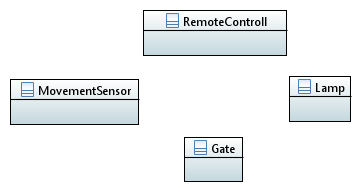
\includegraphics[width=100mm, keepaspectratio]{figures/component.png}
	\caption{Garage gate components}
	\label{fig:Garage Component}
\end{figure}

These components can communicate to each other directly. The possible communication messages is shown on the \figref{Garage communication}.

\begin{figure}[!ht]
	\centering
	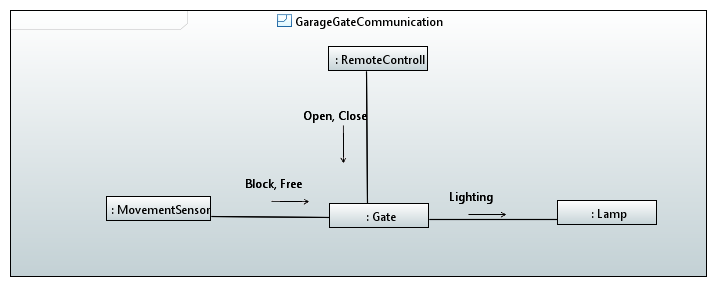
\includegraphics[width=150mm, keepaspectratio]{figures/communication.png}
	\caption{Garage gate communication diagram}
	\label{fig:Garage communication}
\end{figure}

A garage gate fundamentally have 2 main states, the \textit{Opened} and \textit{Closed} states, which is shown below on \figref{Garage Statemachine} figure, with orange colours.  First of all we can start from the \textit{Closed} state, where we can open the gate with an 'open' command. This command sets the state machine in an \textit{Opening} state. While opening the gate, somebody or something can move into the way, so this becomes \textit{Block Opening}. The gate is opening, if the blocking stops. After the \textit{Opening} phase succeeded the gate is \textit{Opened}. In this state we can 'close' the gate with a simple command, and the state machine goes to the \textit{Closing} state. There could be also a blocking action, which stops the closing movement. From this state the gate is starting the closing movement again after a few seconds \textit{Lighting}. When the closing action finished the gate is \textit{Closed}.



\begin{figure}[!ht]
\centering
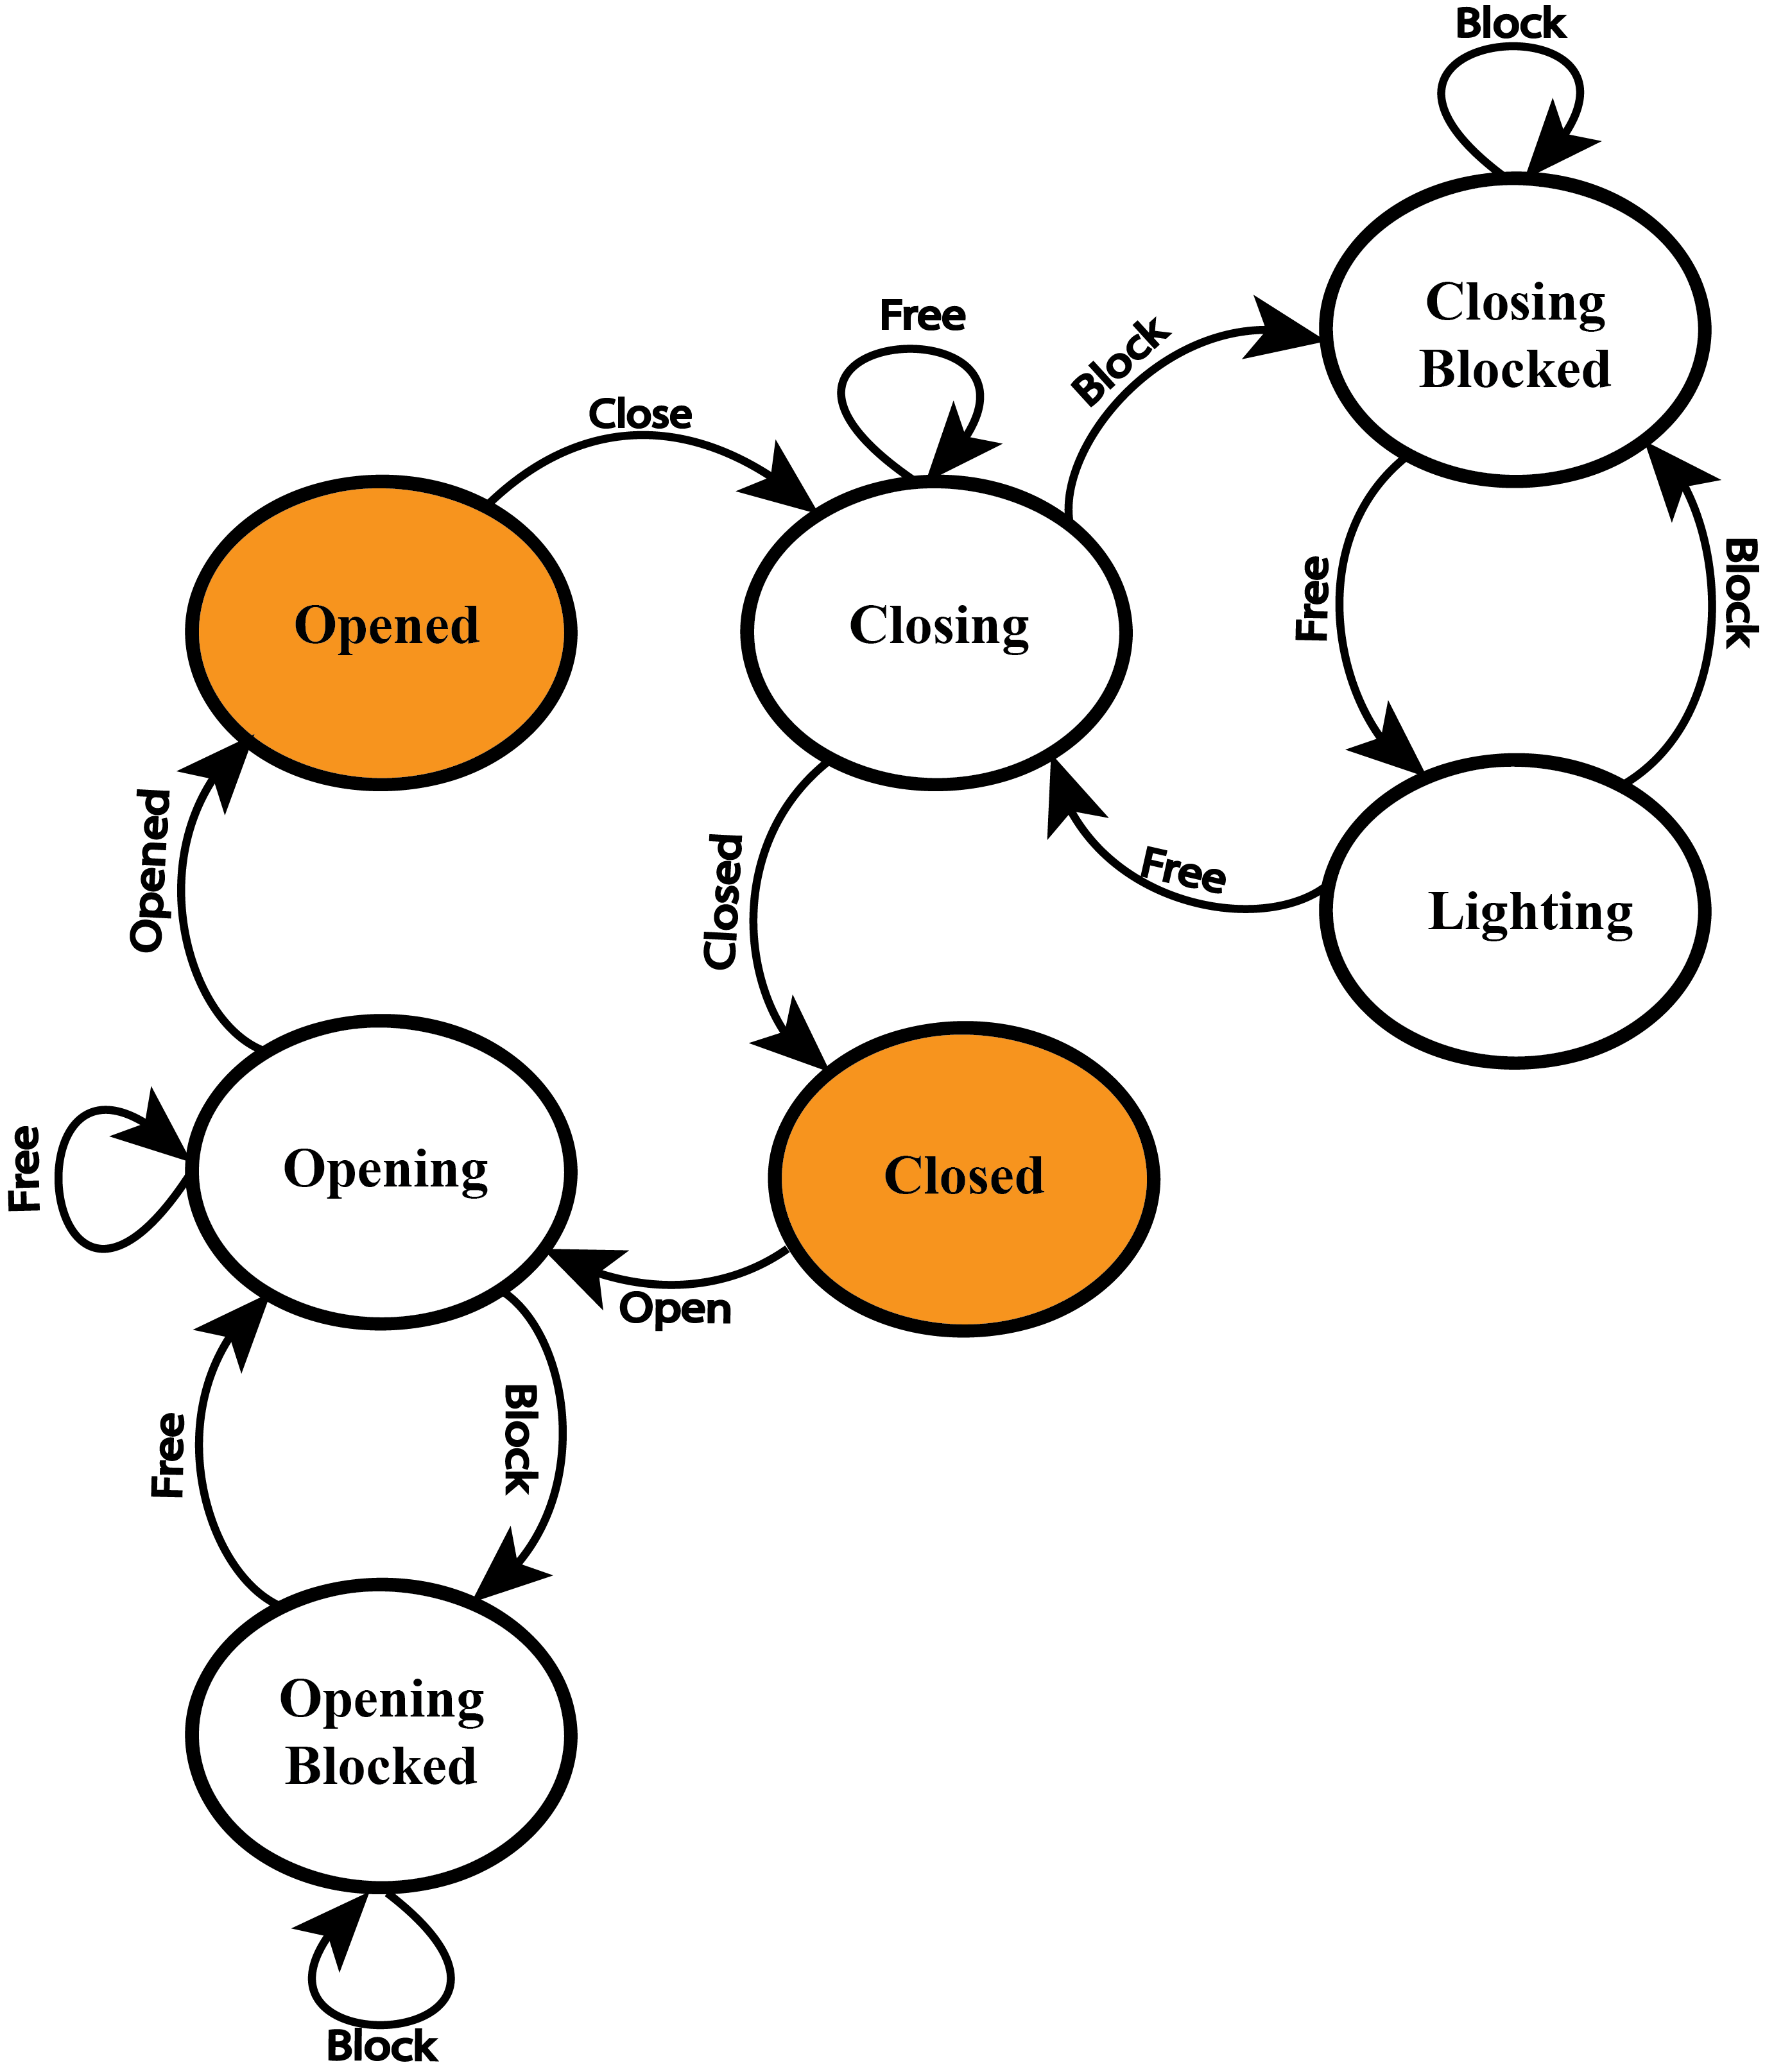
\includegraphics[width=150mm, keepaspectratio]{figures/garageState.png}
\caption{Garage gate state machine diagram}
\label{fig:Garage Statemachine}
\end{figure}

